% !TeX spellcheck = cs_CZ
{\tikzset{external/prefix={tikz/FYZIII/}}
 \tikzset{external/figure name/.add={ch01_}{}}
%---------------------------------------------------------------------------------------------------
% file fyz3ch01.tex
%---------------------------------------------------------------------------------------------------
%====================Kapitola: Elektrostatika ======================================================
\chapter{Elektrostatika}\label{fyz:IIIchapI}
\minitoc

\section{Elektrický náboj}\label{fyz:IIIchapIsecI}
  Jak už bylo řečeno v kapitole \ref{fyz:IIchapI} o elektřině víme, že některá tělesa 
  (například skleněná či ebonitová tyč po předchozím tření) mohou za určitých podmínek silově 
  působit na jiná tělesa. Toto silové působení si vysvětlujeme přítomností elektrických nábojů. 
  Elektrický náboj představuje pro nás výchozí fyzikální veličinu, přičemž mírou jejího množství a 
  rozložení na příslušných tělesech je právě silové působení mezi nimi. Elektrický náboj je 
  veličinou skalární, podobně jako hmotnost, a k jeho určení postačí jediná (reálná) číselná 
  hodnota. Skutečnost, že síly elektrického působení mezi tělesy mohou být jak přitažlivé, tak 
  odpudivé, vysvětlujeme tím, že elektrický náboj může nabývat \emph{kladných} i \emph{záporných} 
  hodnot - tělesa se souhlasným znamením náboje se přitom odpuzují, tělesa s nesouhlasným znamením 
  náboje se přitahují. Tělesa, která nesou elektrický náboj, nazýváme kladně či záporně nabitá, 
  tělesa o nulovém náboji jsou elektricky neutrální, nenabitá. Často se setkáváme s případem, kdy 
  na tělesech jsou odděleně rozloženy kladné a záporné elektrické náboje o téže absolutní hodnotě. 
  Taková tělesa budou také elektricky silově působit, přestože jejich celkový elektrický náboj je 
  nulový. Říkáme jim polarizovaná. 
  
  O přítomnosti elektrického náboje se přesvědčujeme \emph{pouze} na základě jeho 
  \textbf{silového působení}. Znamená to, že existenci jednoho jediného náboje bychom nemohli nijak 
  odhalit. Kdyby existovaly pouze dva náboje, mohli bychom určit, zda jsou souhlasného či 
  nesouhlasného znamení; nemohli bychom však rozhodnout ani o znamení, ani o velikosti těchto 
  nábojů. Teprve jsou-li k dispozici alespoň tři náboje, můžeme jeden z nich vybrat jako jednotkový 
  a kladný a ze silového působení určit velikost a znamení druhých dvou nábojů.
  
  V denním životě se setkávámeN projoevy působení gravitačního a elektromagnetického, které je ze 
  všech nejlépe prozkoumáno. Nejen elektrostatické a elektrodynamické, ale i magnetické, optické, 
  chemické a biologické jevy, chemické vazby a uvolňování chemické energie, mezimolekulární sily 
  podmiňující soudržnost těles, přilnavost a tření, sily svalové kontrakce, tepelné působení 
  slunečního záření a mnoho dalších jevů má svůj původ ve vzájemném působení elektrických nábojů.
  
  Síly elektromagnetického působení mohou být přitažlivé i odpudivé, mohou složitým způsobem 
  záviset na vZdálenosti, směru v prostoru a vzájemné poloze těles, Πa rychlosti jejich pohybu,   
  vlastnostech prostředí, obecně nemusí působit ve směru spojnice interagujících těles, a 
  dokonce nemusí ani splňovat Newtonův zákon akce a reakce.
  
  Elektrický náboj má některé základní vlastnosti, které vyplývají z experimentálních 
  pozorování a uplatňují se i při vzájemné interakci nabitých částic. Tyto vlastností vyjadřuje: 
  
  \begin{enumerate}
    \item \textbf{Zákon zachování náboje}. Elektrický náboj je nestvořitelný a nezničitelný. 
          Jinak řečeno, celkové množství elektrického náboje v elektricky izolované soustavě 
          (jejíž hranicí nemohou procházet náboje) zůstává neměnné. Docházi-li ke srážkám částic, 
          je celkový náboj před reakcí roven celkovëmu naboji po reakci. První experimentální 
          důkaz tohoto zákona podal Faraday v r. 1843 elektrometrickým měřením náboje nabité koule 
          v izolovaném prostoru. Matematické vyjádření tohoto zákona je dáno tzv. \emph{rovnicí 
          kontinuity proudu}, kterou uvedeme v článku ***. %3.1.3. 
    \item \textbf{Zákon invariantnosti náboje}. Velikost elektrického náboje se při pohybu 
          nemění. Jinak řečeno, při všech transformacích vztažné soustavy Zůstává velikost náboje 
          invariantní. Takovou vlastnost má jen málo fyzikálních veličin: například hmotnost  
          částice roste jak známo s rychlostí.
    \item \textbf{Zákon kvantování náboje}. Existuje nejmenší, dále nedělitelný elektrický 
          náboj, který nazýváme elementárním, a všechny elektrické náboje mají velikost, která je 
          jeho celistvým násobkem. Tento atomismus elektřiny souvisí s tím, že elektrický náboj 
          je vlastností částic látky. Velikost elementárního náboje je možné určit pomocí celé 
          řady experimentů, např. klasického Millikanova pokusu (1911), viz článek ***. % 1.1.3
  \end{enumerate}

  Pokud jde o vlastnosti nabitých částic, jsou pozoruhodné ještě dvě okolnosti. Jednou z nich je 
  existence \emph{částic a antičástic}. Ke každé částici existuje antičástice, které se vzájemně 
  liší znamením elektrického náboje\footnote{Částice a antičástice se liší též znaménkem
  magnetického momentu a některých dalších tzv. \emph{kvantových čísel} (leptonový a  baryonový 
  náboj, podivnost, půvab aj.), která charakterizují jejich vzájemné interakce. Existuje několik 
  částic, které jsou se svými antičásticemi totožné (například foton)}. Protože elektrické síly 
  závisejí pouze na souhlasnosti či nesouhlasnosti znamení náboje, mohla by existovat antilátka, 
  kde by nukleony v atomových jádrech byly nahrazeny antinukleony a elektrony atomových obalů svými 
  antičásticemi – pozitrony. Tyto úvahy mají velký význam i pro kosmologii a vyjadřují jednu ze 
  základních symetrií přírody.
  
  Druhá ze zmíněných okolností je \emph{nábojová kvazineutralita} vesmíru. V dostatečně velkých 
  objemech se celkový počet kladných i záporných nábojů vždy vyrovnává a látka, jak se s ní běžně 
  setkáváme v tuhém, kapalném a plynném skupenství, se jeví elektricky neutrální. Odchylky od 
  elektrické neutrality v makroskopických měřítcích se projevují elektrickými silami, které se opět 
  snaží elektrickou neutralitu obnovit.
  
\section{Coulombův zákon}\label{fyz:IIIchapIsecII}
  Při kvantitativním popisu silového působení mezi makroskopickými nabitými tělesy je výhodné v 
  prvním přiblížení abstrahovat od způsobu rozložení náboje v objemu tělesa. Můžeme zavést pojem 
  \textbf{bodového náboje}, který je analogický pojmu hmotného bodu v mechanice. Za bodový náboj 
  můžeme tedy považovat nabité těleso, jehož rozměry jsou zanedbatelně malé ve srovnání se 
  vzdálenostmi, na nichž silové působení uvažujeme. Dvojice bodových nábojů o velikostech, 
  \(Q_1\), \(Q_1\), které jsou umístěny ve vakuu v bodech o polohových vektorech \(\vec{r}_1\), 
  \(\vec{r}_2\) a které jsou nehybné v dané inerciální soustavě souřadnic (obr. \ref{fyz:fig342}), 
  tvoří nejjednodušší makroskopickou soustavu, na níž je možné silové působení mezi náboji 
  studovat. Experimenty tohoto druhu provedl r. 1785 \emph{Ch. A. Coulomb} s použitím 
  \emph{torzních vah}, které představují jeden z nejcitlivějších fyzikálních přístrojů. 

  \begin{figure}[ht!]  %\ref{fyz:fig342}
    \centering
    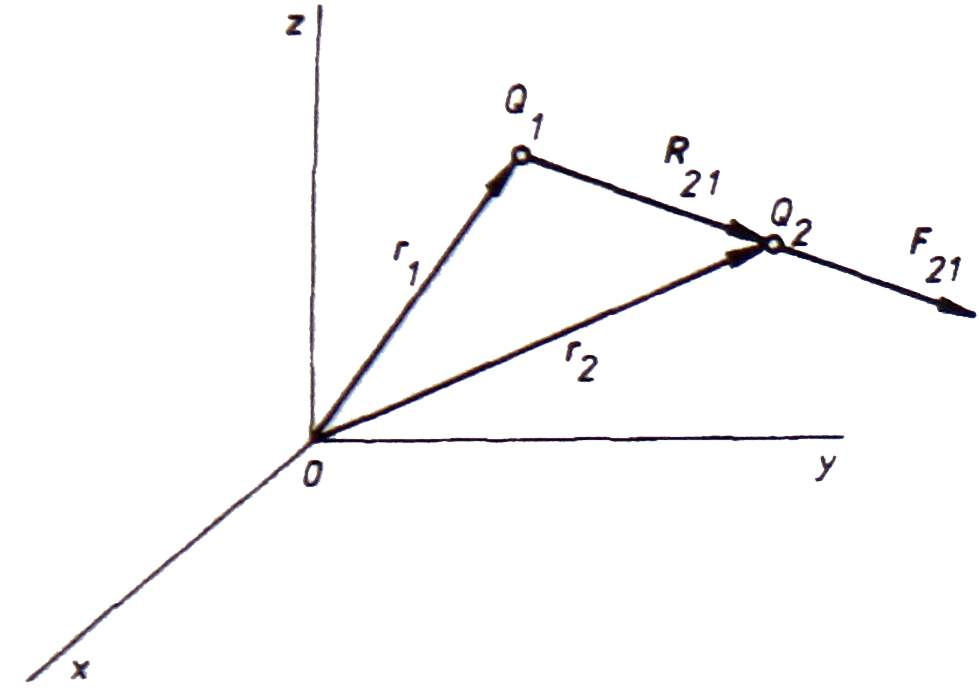
\includegraphics[width=0.8\linewidth]{fyz_fig342.jpg}
    \caption{K vzájemnému silovému působení dvou bodových nábojů
             (\cite[s.~294]{Feynman02}).}
    \label{fyz:fig342}
  \end{figure}

  Sílu působící mezi dvěma malými nabitými kuličkami lze měřit z úhlu zkrutu a dlouhého a tenkého 
  vlákna délky \(l\) a poloměru průřezu \(R\). Úhel \(\alpha\) se zjišťuje odrazem světelného 
  paprsku od zrcátka \(Z\) spojeného s vláknem. Na konci vlákna je zavěšeno vodorovné vahadélko s 
  malými stejnými kuličkami na koncich. Jedna z těchto pohyblivých kuliček nesoucí elektrický 
  náboj \(Q_2\) se ustáli v rovnovážné poloze vůči nehybné kuličce o náboji \(Q_1\) ve 
  vzdálenosti \(R_{12}\) (obr. \ref{fyz:fig343}). Jak uvidíme později, nabitá kulička se navenek 
  chová jakoby elektrický náboj byl umístěn v jejím středu a popsané uspořádání tedy umožňuje 
  měřit síly působící mezi bodovými náboji. Moment \emph{tangenciální síly} \(\vec{F}_t\) se musí 
  rovnat \emph{torznímu momentu} \(\vec{D}\) takže platí

  \begin{equation}\label{fyz:eq372}
    rF_t = D = \frac{\pi}{2}\frac{GR^4}{l}\alpha
  \end{equation}
  kde \(r\) je délka ramene torzních vah, \(G\) modul smyku materiálu vlákna), a tedy
  \begin{equation}\label{fyz:eq373}
    F_{21} = \dfrac{F_t}{\cos\dfrac{\alpha}{2}} = \dfrac{D}{r\cos\dfrac{\alpha}{2}}
  \end{equation}
  
  Na základě výsledků těchto experimentů lze formulovat vztah vyjadřující sílu \(\vec{F}_{12}\), 
  kterou náboj \(Q_1\) působí na náboj \(Q_2\). Tento vztah, známý jako \textbf{Coulombúv zákon}, 
  lze napsat ve tvaru
  \begin{equation}\label{fyz:eq374}
    \vec{F}_{21} = k\frac{Q_1Q_2}{R_{21}^3}\vec{R}_{12}
  \end{equation}
  v němž \(\vec{R}_{21} = \vec{r}_2 - \vec{r}_1\) a \(R_{21}\) je velikost vektoru 
  \(\vec{R}_{21}\). Obráceně sílu \(\vec{F}_{12}\), kterou působí náboj \(Q_2\) na náboj \(Q_1\), 
  dostaneme záměnou indexů \(1\) a \(2\) ve vztahu (\ref{fyz:eq374}). Platí tedy \(\vec{F}_{21} = 
  -\vec{F}_{12}\) v souladu s \emph{Newtonovým principem akce a reakce}. Síly mezi bodovými 
  náboji působí podél jejich spojnice - takové síly nazýváme \emph{centrálními}. Změní-li se 
  znaménko součinu \(Q_1Q_2\), změní se pouze směr síly a nikoli její velikost. Kladné znaménko 
  tohoto součinu odpovídá přitom síle odpudivé, záporné znaménko síle přitažlivé. 
    
  \begin{figure}[ht!]  %\ref{fyz:fig343}
    \centering
    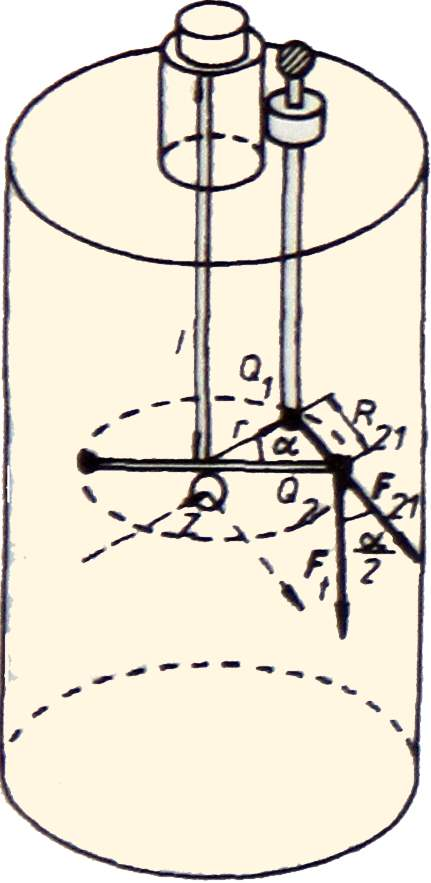
\includegraphics[width=0.5\linewidth]{fyz_fig343.jpg}
    \caption{Coulombovy torzní váhy
             (\cite[s.~294]{Feynman02}).}
    \label{fyz:fig343}
  \end{figure}
  
  Velikost síly působící mezi dvojicí bodových nábojů je rovna
  \begin{equation}\label{fyz:eq375}
    F = \abs{\vec{F}_{21}} = \abs{\vec{F}_{12}} = k\frac{\abs{Q_1Q_2}}{R_{21}^2}
  \end{equation}
  Tato velikost klesá se čtvercem vzdálenosti obou nábojů (stejně jako gravitační působení dvou 
  hmotných bodů) a nezávisí na směru v prostoru. Coulombovy síly jsou tedy izotropní.
  
  Všimneme si nyní poněkud obecnější úlohy. Předpokládejme, že v bodech o polohových vektorech 
  \(\vec{r}_1, \vec{r}_2, \ldots, \vec{r}_N\) jsou rozloženy bodové náboje \(Q_l, Q_2, \ldots, 
  Q_N\). Nechť dále v bodě o polohovém vektoru \(\vec{r}\) je umístěn bodový náboj \(Q\). Ptáme se, 
  jaká síla \(\vec{F}\) bude na náboj \(Q\) působit. Abychom na tuto otázku mohli odpovědět, musíme 
  vědět, jak se změní silové působení mezi dvojicí bodových nábojů, budou-li v prostoru rozmístěny 
  ještě náboje další. 
  
  Experimentální zkušenost ukazuje, že silové působení mezi danou dvojicí nábojů je na přítomnosti 
  dalších nábojů nezávislé. Podle \emph{věty o skládání sil}, známé z mechaniky, můžeme proto 
  celkovou sílu \(\vec{F}\) působící na náboj \(Q\) vyjádřit jako vektorový součet sil 
  \(\vec{F}_i\) (\(i = 1, \ldots,N\)) vyvolaných jednotlivými náboji \(Q_1\) až \(Q_N\). Podle 
  (\ref{fyz:eq374}) bude tedy platit
   
%\section{Urychlování částic indukovaným polem. Betatron}\label{fyz:IIchapXVIIsecIII}
%
%
%\section{Paradox}\label{fyz:IIchapXVIIsecIV}
%
%\section{Generátor střídavého proudu}\label{fyz:IIchapXVIIsecV}
%
%\section{Vzájemná indukčnost}\label{fyz:IIchapXVIIsecVI}
%
%\section{Samoindukčnost}\label{fyz:IIchapXVIIsecVII}
%
%\section{Indukčnost a magnetická energie}\label{fyz:IIchapXVIIsecVIII}
%
%  \begin{figure}[ht!]  %\ref{fyz:fig342}
%    \centering
%    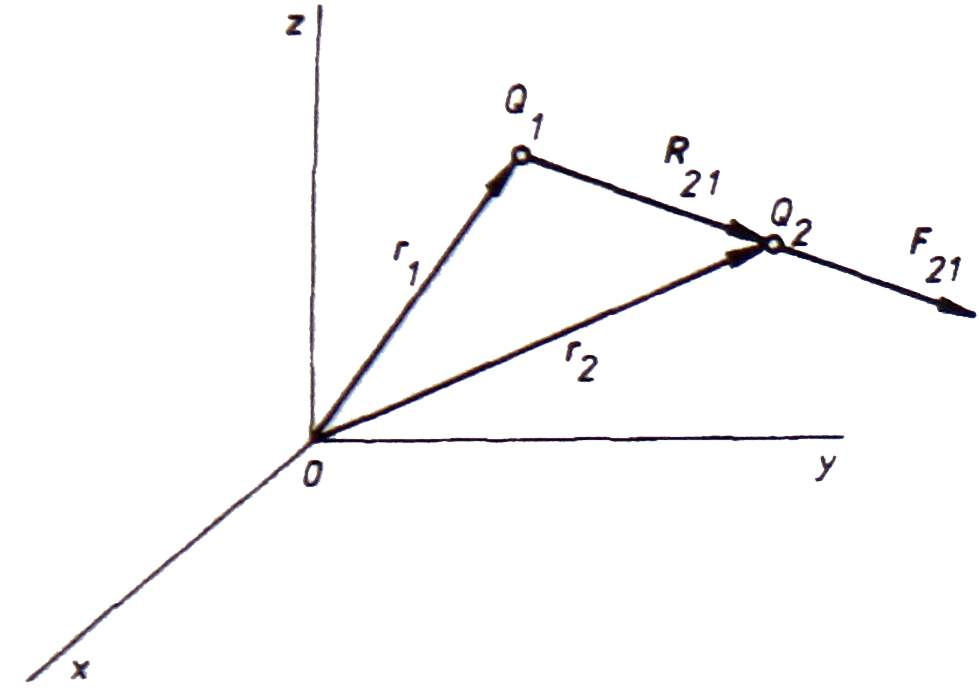
\includegraphics[width=0.8\linewidth]{fyz_fig342.pdf}
%    \caption{Mění-li se v důsledku změny plochy obvodu magnetický tok, indukuje se ve 
%smyčce emn. 
%             (\cite[s.~294]{Feynman02}).}
%    \label{fyz:fig342}
%  \end{figure}
%
%  \begin{figure}[hb!]
%    \centering
%    \begin{tabular}{c}
%     \subfloat[ ]{\label{fyz:fig335a}
%       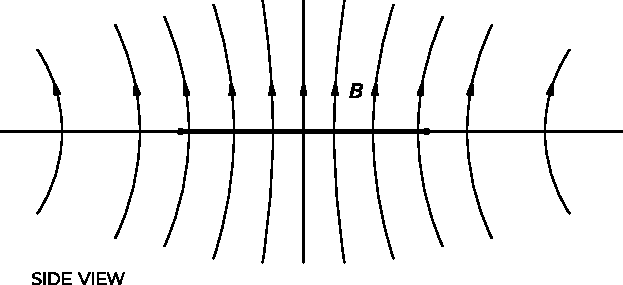
\includegraphics[width=0.45\linewidth]{fyz_fig335a.pdf}}              \\
%     \subfloat[ ]{\label{fyz:fig335b}
%       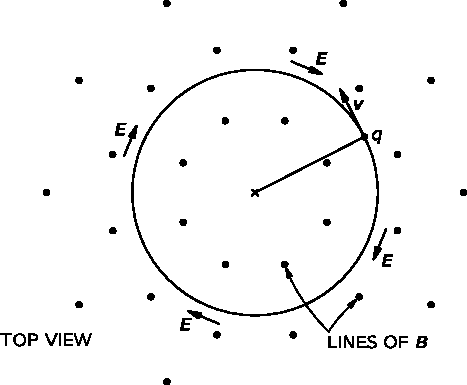
\includegraphics[width=0.45\linewidth]{fyz_fig335b.pdf}}
%    \end{tabular}
%    \caption{Elektron je urychlován v osově symetrické časově proměnném magnetickém poli
%             (\cite[s.~297]{Feynman02}).}
%    \label{fyz:fig335}
%  \end{figure}


  
} %tikzset
%~~~~~~~~~~~~~~~~~~~~~~~~~~~~~~~~~~~~~~~~~~~~~~~~~~~~~~~~~~~~~~~~~~~~~~~~~~~~~~~~~~~~~~~~~~~~~~~~~~
\printbibliography[title={Seznam literatury}, heading=subbibliography]
\addcontentsline{toc}{section}{Seznam literatury}